\documentclass[tikz,border=10pt]{standalone}

% TikZ libraries
\usepackage{tikz}
\usetikzlibrary{arrows.meta, positioning, shapes.geometric, calc, decorations.pathreplacing, patterns, shadows, fit, backgrounds}

% Math and fonts
\usepackage{amsmath, amssymb}
\usepackage{lmodern}

\begin{document}

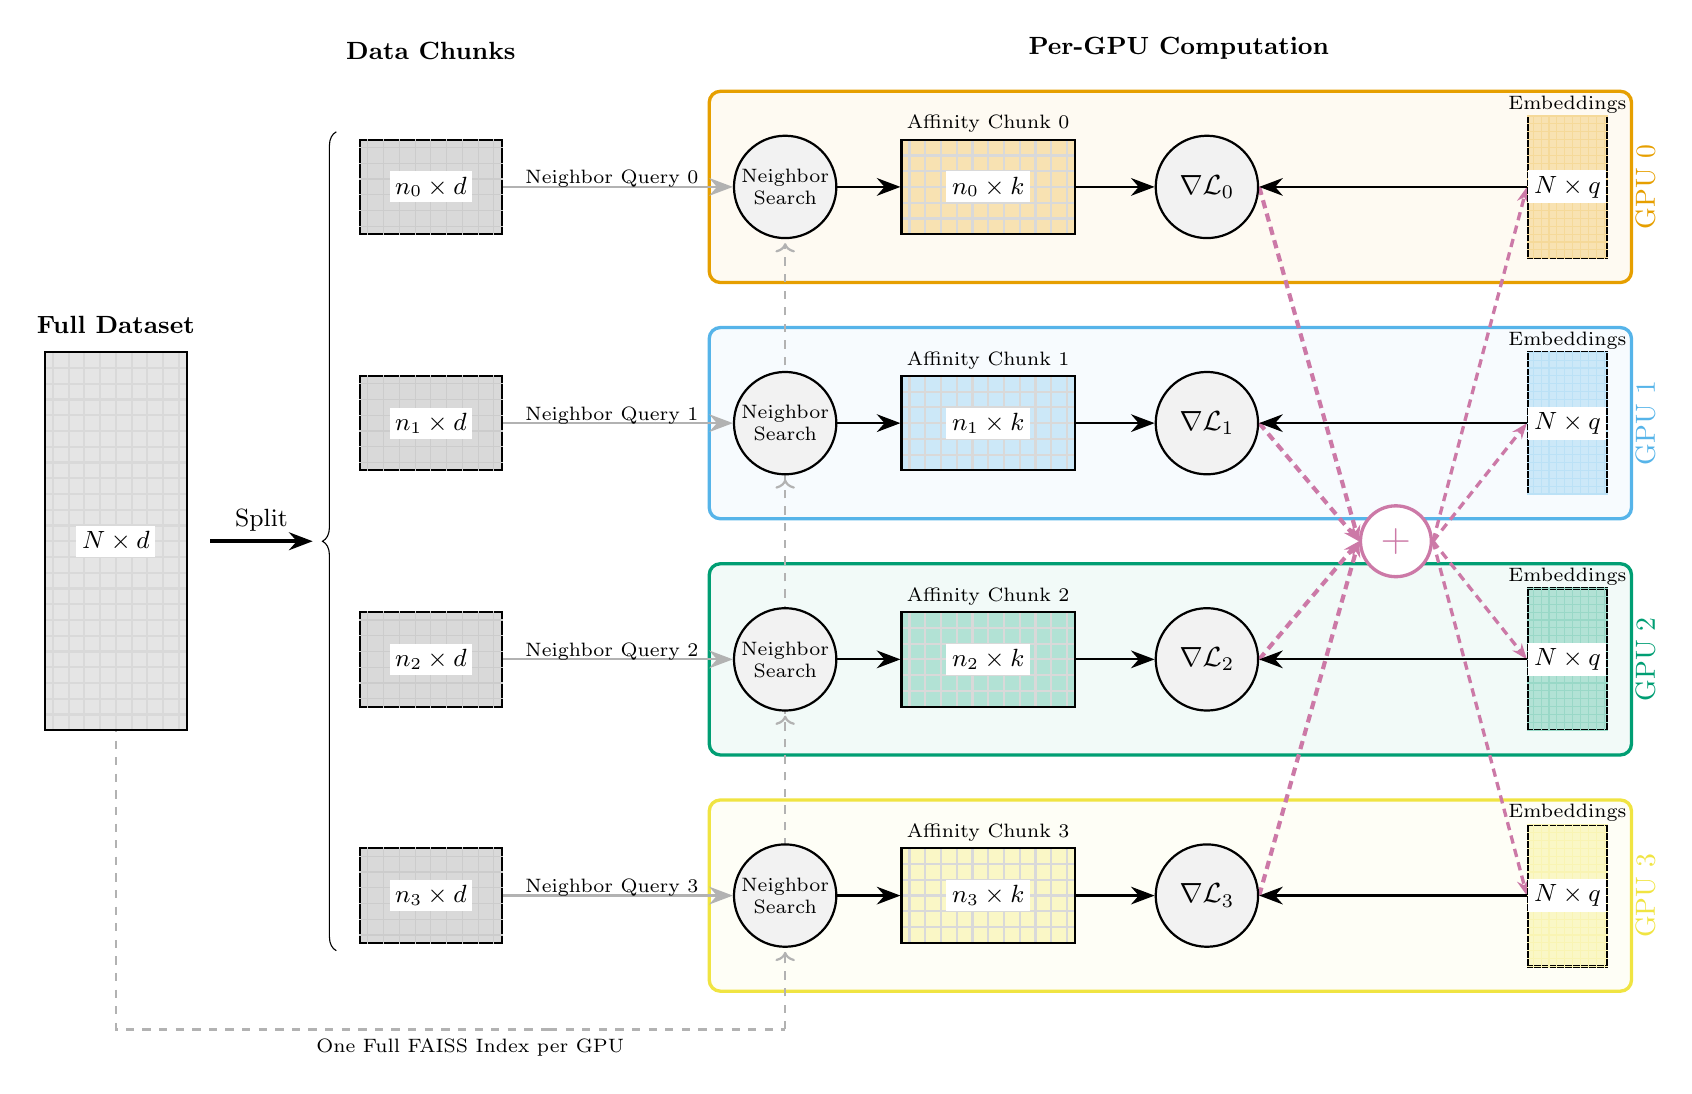
\begin{tikzpicture}[
    gpu/.style={rectangle, draw=black, thick, minimum width=1cm, minimum height=0.8cm, fill=gray!20},
    chunk/.style={rectangle, draw=black, thick, minimum width=1.8cm, minimum height=1.2cm},
    databox/.style={rectangle, draw=black, thick},
    arrow/.style={-{Stealth[length=3mm]}, thick},
    label/.style={font=\small},
    matrix/.style={rectangle, draw=black, thick, path picture={
        \draw[gray!30, step=2mm] (path picture bounding box.south west) grid (path picture bounding box.north east);
    }}
]

% Define colors for each GPU
\definecolor{gpu0color}{RGB}{230, 159, 0}   % Orange
\definecolor{gpu1color}{RGB}{86, 180, 233}  % Sky Blue
\definecolor{gpu2color}{RGB}{0, 158, 115}   % Green
\definecolor{gpu3color}{RGB}{240, 228, 66}  % Yellow
\definecolor{synccolor}{RGB}{204, 121, 167} % Mauve/Purple for gradient sync

% FAR LEFT: Full Data Matrix
\node[chunk, matrix, fill=gray!20, minimum width=1.8cm, minimum height=4.8cm] (fulldata) at (-8, 0) {};
\node[font=\small, fill=white, inner sep=2pt] at (fulldata.center) {$N \times d$};
\node[label, above=0.1cm of fulldata] {\textbf{Full Dataset}};

% Arrow from full data to split chunks (centered with equal spacing)
\draw[arrow, line width=1.5pt] (-6.8, 0) -- (-5.5, 0);
\node[label, font=\small, above] at (-6.15, 0) {Split};

% LEFT SIDE: Dataset Split into Chunks (CPU - grey)
\node[label, above] at (-4, 6.0) {\textbf{Data Chunks}};

% Full dataset divided into 4 chunks with grey fill and grid pattern (on CPU)
\node[chunk, fill=gray!30] (data0) at (-4, 4.5) {};
\draw[gray!40, step=2mm] (data0.south west) grid (data0.north east);
\node[font=\small, fill=white, inner sep=2pt] at (data0.center) {$n_0 \times d$};

\node[chunk, fill=gray!30] (data1) at (-4, 1.5) {};
\draw[gray!40, step=2mm] (data1.south west) grid (data1.north east);
\node[font=\small, fill=white, inner sep=2pt] at (data1.center) {$n_1 \times d$};

\node[chunk, fill=gray!30] (data2) at (-4, -1.5) {};
\draw[gray!40, step=2mm] (data2.south west) grid (data2.north east);
\node[font=\small, fill=white, inner sep=2pt] at (data2.center) {$n_2 \times d$};

\node[chunk, fill=gray!30] (data3) at (-4, -4.5) {};
\draw[gray!40, step=2mm] (data3.south west) grid (data3.north east);
\node[font=\small, fill=white, inner sep=2pt] at (data3.center) {$n_3 \times d$};

% Brace showing chunks come from full dataset
\draw[decorate, decoration={brace, amplitude=5pt, mirror}]
    (-5.2, 5.2) -- (-5.2, -5.2);

% Center point for the full dataset used to build each rank-local FAISS index
\coordinate (faiss_center) at (-8, 0);

% RIGHT SIDE: GPU Processing
\node[label, above] at (5.5, 6.0) {\textbf{Per-GPU Computation}};

% Y positions for each GPU row (increased spacing to avoid overlap)
\foreach \i/\col/\ypos/\nsize in {0/gpu0color/4.5/n_0, 1/gpu1color/1.5/n_1, 2/gpu2color/-1.5/n_2, 3/gpu3color/-4.5/n_3} {

    % Neighbor Search operation (moved closer to data chunks)
    \node[circle, draw=black, thick, minimum size=1.3cm, fill=gray!10] (search\i) at (0.5, \ypos) {};
    \node[font=\scriptsize, align=center] at (search\i.center) {Neighbor\\Search};

    % Output (affinity matrix slice) - wider matrix
    \node[matrix, fill=\col!30, minimum width=2.2cm, minimum height=1.2cm, right=0.8cm of search\i] (output\i) {};
    \node[font=\small, fill=white, inner sep=2pt] at (output\i.center) {$\nsize \times k$};
    \node[label, above=-0.05cm of output\i, font=\scriptsize] {Affinity Chunk \i};

    % Gradient Module (increased spacing from affinity)
    \node[circle, draw=black, thick, minimum size=1.3cm, fill=gray!10, right=1.0cm of output\i] (grad\i) {};
    \node[font=\normalsize, align=center] at (grad\i.center) {$\nabla \mathcal{L}_\i$};

    % Embeddings (N × q) - tall and narrow with dense grid (spacing from gradient)
    \node[rectangle, draw=black, thick, fill=\col!30, minimum width=1cm, minimum height=1.8cm, right=3.4cm of grad\i] (embed\i) {};
    \draw[\col!40, step=1mm] (embed\i.south west) grid (embed\i.north east);
    \node[font=\small, fill=white, inner sep=2pt] at (embed\i.center) {$N \times q$};
    \node[label, above=-0.10cm of embed\i, font=\scriptsize] {Embeddings};

    % Arrow from search to output
    \draw[arrow] (search\i.east) -- (output\i.west);

    % Arrow from affinity to gradient
    \draw[arrow] (output\i.east) -- (grad\i.west);

    % Arrow from embeddings to gradient
    \draw[arrow] (embed\i.west) -- (grad\i.east);
}

% Draw GPU boxes and FAISS index arrows in background layer
\begin{pgfonlayer}{background}
    % GPU boxes (now including gradient and embeddings)
    \node[draw=gpu0color, very thick, fill=gpu0color!5, rounded corners, fit=(search0)(output0)(grad0)(embed0), inner sep=0.3cm, label={[font=\small]above left:GPU 0}] (gpubox0) {};
    \node[draw=gpu1color, very thick, fill=gpu1color!5, rounded corners, fit=(search1)(output1)(grad1)(embed1), inner sep=0.3cm, label={[font=\small]above left:GPU 1}] (gpubox1) {};
    \node[draw=gpu2color, very thick, fill=gpu2color!5, rounded corners, fit=(search2)(output2)(grad2)(embed2), inner sep=0.3cm, label={[font=\small]above left:GPU 2}] (gpubox2) {};
    \node[draw=gpu3color, very thick, fill=gpu3color!5, rounded corners, fit=(search3)(output3)(grad3)(embed3), inner sep=0.3cm, label={[font=\small]above left:GPU 3}] (gpubox3) {};

    % Full-dataset flow used to build one complete FAISS index per GPU.
    % These dashed arrows represent replication, not a shared index.
    % Horizontal backbone below all FAISS search modules
    \coordinate (backbone_start) at (-2.5, -6.2);
    \coordinate (backbone_end) at (0.5, -6.2);

    % Draw from the full dataset down and right to the replication backbone
    \draw[thick, dashed, gray!60] (faiss_center) |- (backbone_start);

    % Draw horizontal backbone
    \draw[thick, dashed, gray!60] (backbone_start) -- (backbone_end);
    \node[font=\scriptsize, black, below] at (-3.5, -6.2) {One Full FAISS Index per GPU};

    % Draw vertical connections to each rank-local FAISS search
    \foreach \i in {0,1,2,3} {
        \coordinate (connect\i) at (search\i |- backbone_end);
        \draw[->, thick, dashed, gray!60] (connect\i) -- ($(search\i.south) + (0, -0.05)$);
    }
\end{pgfonlayer}

% Arrows from data chunks to FAISS Search (grey - data stays on CPU, accessed by GPU)
\draw[arrow, gray!60] (data0.east) -- (search0.west);
\node[font=\scriptsize, black] at (-1.7, 4.6) {Neighbor Query 0};

\draw[arrow, gray!60] (data1.east) -- (search1.west);
\node[font=\scriptsize, black] at (-1.7, 1.6) {Neighbor Query 1};

\draw[arrow, gray!60] (data2.east) -- (search2.west);
\node[font=\scriptsize, black] at (-1.7, -1.4) {Neighbor Query 2};

\draw[arrow, gray!60] (data3.east) -- (search3.west);
\node[font=\scriptsize, black] at (-1.7, -4.4) {Neighbor Query 3};

% GPU labels on the right side of boxes
\node[font=\normalsize, gpu0color, right=0.4cm of gpubox0.east, rotate=90, anchor=south] {GPU 0};
\node[font=\normalsize, gpu1color, right=0.4cm of gpubox1.east, rotate=90, anchor=south] {GPU 1};
\node[font=\normalsize, gpu2color, right=0.4cm of gpubox2.east, rotate=90, anchor=south] {GPU 2};
\node[font=\normalsize, gpu3color, right=0.4cm of gpubox3.east, rotate=90, anchor=south] {GPU 3};

% GRADIENT SYNCHRONIZATION
% Single central sum node (positioned in the center of grad-embed space)
\node[circle, draw=synccolor, very thick, minimum size=0.9cm, fill=white] (sumnode) at ($(grad1)!0.5!(grad2) + (2.4, 0)$) {};
\node[font=\Large, synccolor] at (sumnode.center) {$+$};

% Arrows from all gradients to central sum (dashed with smaller arrowheads, in background, starting from east/right side)
\begin{pgfonlayer}{background}
    \draw[-{Stealth[length=2mm]}, synccolor, line width=1.5pt, dash pattern=on 3pt off 2pt] (grad0.east) -- (sumnode.west);
    \draw[-{Stealth[length=2mm]}, synccolor, line width=1.5pt, dash pattern=on 3pt off 2pt] (grad1.east) -- (sumnode.west);
    \draw[-{Stealth[length=2mm]}, synccolor, line width=1.5pt, dash pattern=on 3pt off 2pt] (grad2.east) -- (sumnode.west);
    \draw[-{Stealth[length=2mm]}, synccolor, line width=1.5pt, dash pattern=on 3pt off 2pt] (grad3.east) -- (sumnode.west);

    % Arrows from central sum to all embeddings (dashed with smaller arrowheads, straight lines, in background to avoid overlap)
    \draw[-{Stealth[length=2mm]}, synccolor, line width=1.2pt, dash pattern=on 3pt off 2pt] (sumnode.east) -- (embed0.west);
    \draw[-{Stealth[length=2mm]}, synccolor, line width=1.2pt, dash pattern=on 3pt off 2pt] (sumnode.east) -- (embed1.west);
    \draw[-{Stealth[length=2mm]}, synccolor, line width=1.2pt, dash pattern=on 3pt off 2pt] (sumnode.east) -- (embed2.west);
    \draw[-{Stealth[length=2mm]}, synccolor, line width=1.2pt, dash pattern=on 3pt off 2pt] (sumnode.east) -- (embed3.west);
\end{pgfonlayer}

\end{tikzpicture}

\end{document}
